\documentclass[12pt, a4paper, DIV=12, BCOR=1cm]{scrartcl}
% Liste eingebundener Pakete (kann erweitert werden!)
% in {} steht der Name des Pakets, in [] stehen Optionen
% zu allen Packages gibt eine eine Dokumentation, z.B. auf ctan.org
\usepackage{graphicx}
\usepackage[utf8]{inputenc}
\usepackage[T1]{fontenc}
\usepackage{lmodern}
\usepackage{geometry}
\usepackage[firstpage]{draftwatermark}
\usepackage{amsmath,amssymb}
\usepackage{lmodern}
\usepackage{color}
\usepackage{caption}
\usepackage{graphicx}
\usepackage{float}
\usepackage[ngerman]{babel}
\usepackage{appendix}
\SetWatermarkLightness{1}
\SetWatermarkText{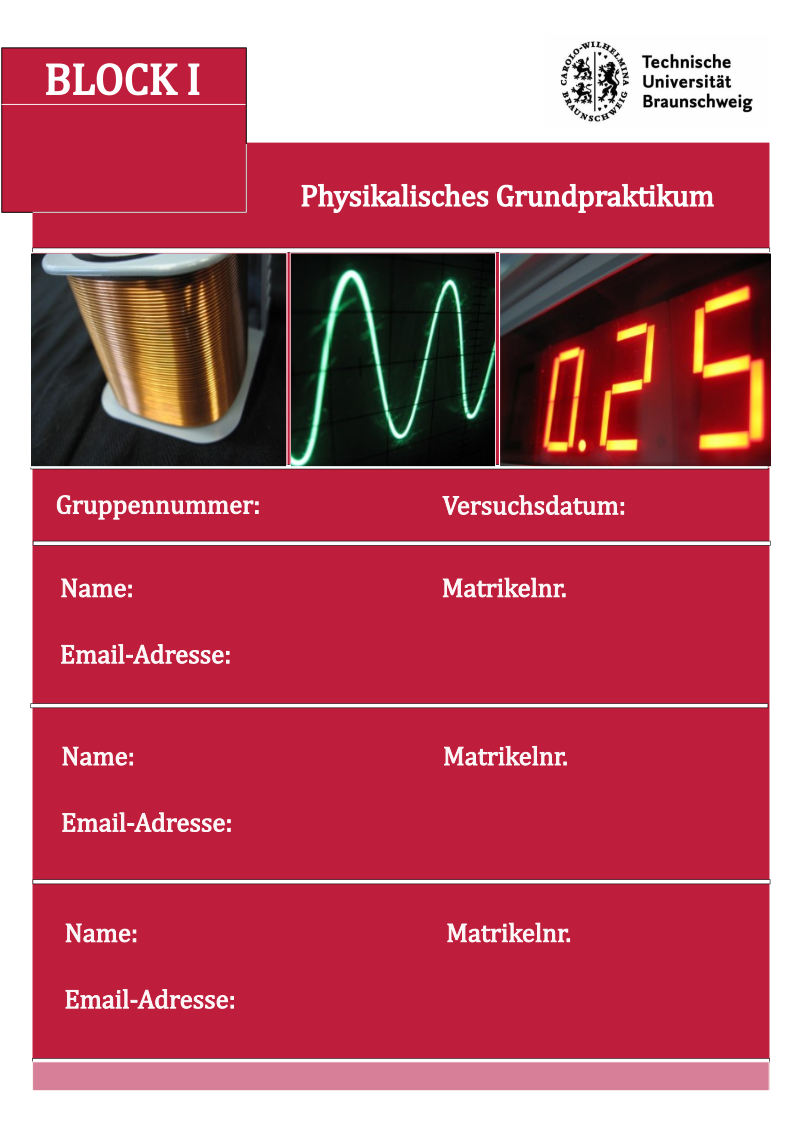
\includegraphics[angle=-45]{Protokolldeckblatt_BlockI_Hintergrund.png}}

\begin{document}
	\thispagestyle{empty}
	\newgeometry{left=0mm, right=0mm,top=0mm,bottom=0mm}
	\vspace*{3.1cm}
	\hspace*{0.9cm}
	\begin{minipage}{2cm}
			{\color{white} \fontsize{48}{40} \selectfont \textbf{V01}} %V11 durch Versuchsnummer ersetzen
	\end{minipage}

	\vspace{8.45cm}
	\hspace*{7cm}
	\begin{minipage}{2cm}
	{\color{white}  \Large \textbf{000}} %Gruppennummer eintragen
	\end{minipage}
	\hspace*{7cm}
	\begin{minipage}{4cm}
	{\color{white}  \Large \textbf{01.01.2001}} %Datum eintragen
    \end{minipage}
    
	\vspace{1.65cm}
	\hspace*{3cm}
	\begin{minipage}{8cm}
	{\color{white}  \Large \textbf{Vorname1 Nachname1}} %Name Partner 1 eintragen
	\end{minipage}
	\hspace*{3.3cm}
	\begin{minipage}{3cm}
	{\color{white}  \Large \textbf{1234567}} %Matrikelnummer von Partner 1
	\end{minipage}
	
	\vspace{1.3cm}
	\hspace*{5.75cm}
	\begin{minipage}{14cm}
	{\color{white}  \Large \textbf{vorname.nachname@tu-braunschweig.de}} %Emailadresse von Partner 1
	\end{minipage}
	
	\vspace{2.15cm}
	\hspace*{3.1cm}
	\begin{minipage}{8cm}
	{\color{white}  \Large \textbf{Vorname1 Nachname1}} %Name Partner 2 eintragen
	\end{minipage}
	\hspace*{3.3cm}
	\begin{minipage}{3cm}
	{\color{white}  \Large \textbf{1234567}} %Matrikelnummer von Partner 2
	\end{minipage}

	\vspace{1.3cm}
	\hspace*{5.75cm}
	\begin{minipage}{14cm}
	{\color{white}  \Large \textbf{vorname.nachname@tu-braunschweig.de}} %Emailadresse von Partner 2
	\end{minipage}
	
\vspace{2.35cm}
\hspace*{3.15cm}
\begin{minipage}{8cm}
	{\color{white}  \Large \textbf{Vorname1 Nachname1}} %Name Partner 3 eintragen, falls kein Partner 3 einfach löschen
\end{minipage}
\hspace*{3.3cm}
\begin{minipage}{3cm}
	{\color{white}  \Large \textbf{1234567}} %Matrikelnummer von Partner 3, falls kein Partner 3, einfach löschen
\end{minipage}

	\vspace{1.3cm}
	\hspace*{5.75cm}
	\begin{minipage}{14cm}
	{\color{white}  \Large \textbf{vorname.nachname@tu-braunschweig.de}} %Emailadresse von Partner 3, falls kein Partner 3, einfach löschen
	\end{minipage}
\restoregeometry
\pagebreak
\tableofcontents
\newpage
\section{Einleitung}
\section{Physikalische Grundlagen}
\subsection{Grundlage 1}
\subsection{Grundlage 2}
\section{Versuchsdurchführung und -auswertung}
\subsection{Versuchsteil 1}
\subsection{Versuchsteil 2}
\subsection{Versuchsteil 3}
\subsection{Zusammenfassung und Fazit}

Hilfreiche Umgebungen:
%Einbindung von Gleichungen
EQUATION-UMGEBUNG:
\begin{equation}
	F = m \cdot a
	\label{Fma}
\end{equation}
%Gleichungen in dieser Umgebung erhalten automatisch eine Gleichungsnummer. Zusätzlich ist die Gleichungsumgebung abgesetzt. Über \ref{...} kann auf diese Gleichungen referenziert werden. Um auf die seite zu verweisen, auf der die Gleichung steht, ist \pageref{...} zu verwenden.

ALIGN-Umgebung:
\begin{align}
	\theta_z &= \int_V \rho (x^2 + y^2)\,dx\,dy\,dz \\
	&=\frac{M}{\pi R^2 h} \int_{-h/2}^{+h/2}{dz} \int_{0}^{2\pi}{d\varphi} \int_{0}^{R}{r^3\,dr} \\
	&= \frac{M}{\pi R^2 h} \cdot h \cdot 2\pi \cdot \frac{1}{4} R^4 \\
	&= \frac{1}{2}MR^2
\end{align}
%Die Align-Umgebung eignet sich für mehrschrittige Umformungen, da sie es erlaubt, die Gleichheitszeichen untereinander anzuordnen.
%
ITEMIZE- und ENUMERATE-Umgebung:
\begin{itemize}
	\item Ein Stichpunkt
	\item Noch ein Stichpunkt
	\item \ldots
\end{itemize}

%Mit \item[label] description kann ein eigenes label statt des standardmäßigen Stichpunkt-Punkts erstellt werden.
%Die \texttt{enumerate}-Umgebung numeriert die einzelnen Stichpunkte. 

\begin{enumerate}
	\item Ein anderer, erster Stichpunkt
	\item Ein anderer, zweiter Stichpunkt
	\item \ldots
\end{enumerate}

TABULAR-Umgebung:
%Erstellung von Tabellen
\begin{table}[h!]
	\centering
	\begin{tabular}{|r|r|r|r|}
		\hline
		$U$ (V) & $\Delta U$ (V) & $I$ (mA) & $\Delta I$ (mA) \\
		\hline
		1.09 & 0.02 & 0.12 & 0.05 \\
		2.04 & 0.02 & 0.23 & 0.05 \\
		3.98 & 0.02 & 0.46 & 0.05 \\
		5.80 & 0.02 & 0.70 & 0.05 \\
		8.07 & 0.02 & 0.94 & 0.05 \\
		9.91 & 0.02 & 1.15 & 0.05 \\
		12.70 & 0.02 & 1.44 & 0.05 \\
		14.99 & 0.02 & 1.74 & 0.05 \\
		\hline
	\end{tabular}
	\caption{Elektrische Stromstärke $I$ als Funktion der anliegenden Spannung $U$ für einen unbekannten Widerstand $R_1$.}
	\label{tab:daten1}
\end{table}

FIGURE-Umgebung:
Einbindung von Graphiken:
\begin{figure}[htb!]
	\centering
	
\includegraphics[width=0.4\linewidth]{TU Logo.jpeg}
	\caption{TU-Logo}
	\label{fig:TU-Logo}
\end{figure}

\newpage

% Beginnt den Anhang
\appendix
\appendixpage
\addappheadtotoc

\section{Messdaten zu Versuchsteil 1}

Manchmal bietet es sich auch an, Tabellen mit Messwerten oder zusätzliche Abbildungen in den Anhang auszulagern.

\begin{table}[ht]
	\centering
	\begin{tabular}{r|r|r|r}
		\hline
		$U$ (V) & $\Delta U$ (V) & $I$ (mA) & $\Delta I$ (mA) \\
		\hline
		1.09 & 0.02 & 0.12 & 0.05 \\
		2.04 & 0.02 & 0.23 & 0.05 \\
		3.98 & 0.02 & 0.46 & 0.05 \\
		5.80 & 0.02 & 0.70 & 0.05 \\
		8.07 & 0.02 & 0.94 & 0.05 \\
		9.91 & 0.02 & 1.15 & 0.05 \\
		12.70 & 0.02 & 1.44 & 0.05 \\
		14.99 & 0.02 & 1.74 & 0.05 \\
		\hline
	\end{tabular}
	\caption{Elektrische Stromstärke $I$ als Funktion der anliegenden Spannung $U$ für einen unbekannten Widerstand $R_1$.}
	\label{tab:datenanhang1}
\end{table}
\end{document}